
\chapter{Compiler}

\section{Development Environment}

\paragraph{} The BigDuck compiler will be developed using the Go programming
language. Antlr4 will be used as lexer and parser generator. And it will be
developed on MacOS, any other system support is not considered. Nevertheless
with access to a Go compiler and ANTLR, it should be possible to run the
BigDuck compiler however this has not been tested.

\section{Lexical Analisis}

\subsubsection{Reserved Keywords}
\begin{verbatim}
proc    return  if      else    loop    break   skip    and
or      not     var     int     float   bool    true    false
print   read    sin     asin    cos     acos    tan     atan
atan2   exp     exp     ln      sqrt    pow     mod     abs
ceil    floor   mean    median  mode
\end{verbatim}

\subsubsection{Tokens}
\begin{align*}
	\texttt{DIGITS}
	&\rightarrow\texttt{[0-9]+}\\
	\texttt{LETTER}
	&\rightarrow\texttt{[A-Za-z]}\\
	\texttt{SIGN}
	&\rightarrow\texttt{`` - ''}\\
	\texttt{CTE\_INT}
	&\rightarrow\texttt{sign? digits}\\
	\texttt{CTE\_FLOAT}
	&\rightarrow\texttt{sign? digits (\textbackslash.\ digits)?}\\
	\texttt{ID}
	&\rightarrow\texttt{letter (letter | [0-9] | `` \_ '')*}\\
	\texttt{COMMENT}
	&\rightarrow\texttt{`` \#| '' \phantom{}.*? `` |\# '' *}\\
\end{align*}

\section{Syntactical Analisis}
\paragraph{Note} The following grammar is not a one-to-one description of the
grammar used in the compiler, this is because there are addtional rules just to
have some breakpoints on the grammar required for compilation.
\begin{align*}
	\texttt{program}
	\rightarrow&\ \texttt{vars\_decl procs\_decl}\\
	\phantom{0}\\
	\texttt{vars\_decl}
	\rightarrow&\ \texttt{var\_decl var\_decl}\\
            |&\ \epsilon\\
	\texttt{var\_decl}
	\rightarrow&\ \texttt{VAR ID next\_var var\_type `` ; '' next\_var\_decl}\\
	\texttt{next\_var}
	\rightarrow&\ \texttt{`` , '' ID next\_var}\\
            |&\ \epsilon\\
	\texttt{next\_var\_decl}
	\rightarrow&\ \texttt{var\_decl next\_var\_decl}\\
            |&\ \epsilon\\
	\phantom{0}\\
	\texttt{var\_type}
	\rightarrow&\ \texttt{scalar | tensor}\\
	\phantom{0}\\
	\texttt{scalar}
	\rightarrow&\ \texttt{INT | FLOAT | BOOL}\\
	\phantom{0}\\
	\texttt{tensor}
	\rightarrow&\ \texttt{dimension scalar}\\
	\texttt{dimension}
	\rightarrow&\ \texttt{`` [ '' num\_expr `` ] next\_dimension ''}\\
	\texttt{next\_dimension}
	\rightarrow&\ \texttt{dimension next\_dimension}\\
            |&\ \epsilon\\
	\phantom{0}\\
	\texttt{procs\_decl}
	\rightarrow&\ \texttt{proc\_decl procs\_decl}\\
            |&\ \epsilon\\
	\phantom{0}\\
	\texttt{proc\_decl}
	\rightarrow&\ \texttt{PROC ID proc\_args ret\_type local\_decl block}\\
	\phantom{0}\\
	\texttt{proc\_args}
	\rightarrow&\ \texttt{`` ( '' `` ) ''}\\
            |&\ \texttt{`` ( '' ID next\_args scalar next\_types `` ) ''}\\
	\texttt{next\_args}
	\rightarrow&\ \texttt{`` , '' ID next\_args}\\
            |&\ \epsilon\\
	\texttt{next\_types}
	\rightarrow&\ \texttt{`` ; '' ID next\_args scalar next\_types}\\
            |&\ \epsilon\\
\end{align*}

\begin{align*}
	\texttt{ret\_type}
	\rightarrow&\ \texttt{`` -> '' scalar}\\
            |&\ \epsilon\\
	\phantom{0}\\
	\texttt{bool\_expr}
	\rightarrow&\ \texttt{and\_expr next\_bool}\\
	\texttt{next\_bool}
	\rightarrow&\ \texttt{OR bool\_expr}\\
            |&\ \epsilon\\
	\phantom{0}\\
	\texttt{and\_expr}
	\rightarrow&\ \texttt{not\_expr next\_and}\\
	\texttt{next\_and}
	\rightarrow&\ \texttt{AND bool\_expr}\\
            |&\ \epsilon\\
	\phantom{0}\\
	\texttt{not\_expr}
	\rightarrow&\ \texttt{(NOT | } \epsilon \texttt{ ) bool\_term}\\
	\texttt{bool\_term}
	\rightarrow&\ \texttt{`` ( '' bool\_expr `` ) ''}\\
            |&\ \texttt{rel\_expr}\\
            |&\ \texttt{TRUE}\\
            |&\ \texttt{FALSE}\\
            |&\ \texttt{variable}\\
            |&\ \texttt{proc\_call}\\
	\phantom{0}\\
	\texttt{rel\_expr}
	\rightarrow&\ \texttt{num\_expr rel\_op num\_expr}\\
	\texttt{rel\_op}
	\rightarrow&\ \texttt{`` = ''}\\
            |&\ \texttt{`` /= ''}\\
            |&\ \texttt{`` < ''}\\
            |&\ \texttt{`` > ''}\\
            |&\ \texttt{`` >= ''}\\
            |&\ \texttt{`` <= ''}\\
	\phantom{0}\\
	\texttt{num\_expr}
	\rightarrow&\ \texttt{prod\_expr next\_sum}\\
	\texttt{next\_sum}
	\rightarrow&\ \texttt{( `` + '' | `` - '') num\_expr}\\
            |&\ \epsilon\\
	\phantom{0}\\
	\texttt{prod\_expr}
	\rightarrow&\ \texttt{factor next\_prod}\\
	\texttt{next\_prod}
	\rightarrow&\ \texttt{(`` * '' | `` / '') prod\_expr}\\
            |&\ \epsilon\\
\end{align*}

\begin{align*}
	\texttt{factor}
	\rightarrow&\ \texttt{`` ( '' num\_expr `` ) ''}\\
            |&\ \texttt{CTE\_INT}\\
            |&\ \texttt{CTE\_FLOAT}\\
            |&\ \texttt{variable}\\
            |&\ \texttt{proc\_call}\\
            |&\ \texttt{functions}\\
	\phantom{0}\\
	\texttt{variable}
            |&\ \texttt{ID (dimension | } \epsilon \texttt{ )}\\
	\phantom{0}\\
	\texttt{proc\_call}
	\rightarrow&\ \texttt{ID `` ( '' (param | } \epsilon \texttt{ ) `` ) ''}\\
	\texttt{param}
	\rightarrow&\ \texttt{param\_term next\_param}\\
	\texttt{param\_term}
	\rightarrow&\ \texttt{bool\_expr}\\
            |&\ \texttt{num\_expr}\\
	\texttt{next\_param}
	\rightarrow&\ \texttt{`` , '' param}\\
	\texttt{block}
	\rightarrow&\ \texttt{`` \{ '' stmts `` \} ''}\\
	\phantom{0}\\
	\texttt{stmts}
	\rightarrow&\ \texttt{stmt stmts}\\
            |&\ \epsilon\\
	\texttt{stmt}
	\rightarrow&\ \texttt{assigment  `` ; ''}\\
            |&\ \texttt{condition}\\
            |&\ \texttt{loop\_stmt}\\
            |&\ \texttt{ctrl\_flow `` ; ''}\\
            |&\ \texttt{ret\_stmt `` ; ''}\\
            |&\ \texttt{proc\_call `` ; ''}\\
            |&\ \texttt{built\_in `` ; ''}\\
	\phantom{0}\\
	\texttt{assignment}
	\rightarrow&\ \texttt{variable `` <- '' (num\_expr | bool\_expr)}\\
	\phantom{0}\\
	\texttt{condition}
	\rightarrow&\ \texttt{IF bool\_expr block (alter | } \epsilon \texttt{ )}\\
	\phantom{0}\\
	\texttt{alter}
	\rightarrow&\ \texttt{IF bool\_expr block (alter | } \epsilon \texttt{ )}\\
	\phantom{0}\\
	\texttt{loop}
	\rightarrow&\ \texttt{LOOP (for\_style | while\_style | infinite) block}\\
	\texttt{for\_style}
	\rightarrow&\ \texttt{
            (assignment | } \epsilon \texttt{ ) 
            `` ; '' bool\_expr `` ; '' assignment }\\
	\texttt{while\_style}
	\rightarrow&\ \texttt{bool\_expr}\\
	\texttt{infinite}
	\rightarrow&\ \epsilon\\
\end{align*}

\begin{align*}
	\texttt{built\_in}
	\rightarrow&\ \texttt{print}\\
            |&\ \texttt{read}\\
	\phantom{0}\\
	\texttt{functions}
	\rightarrow&\ \texttt{u\_func}\\
            |&\ \texttt{bin\_func}\\
            |&\ \texttt{vec\_func}\\
	\phantom{0}\\
	\texttt{print}
	\rightarrow&\ \texttt{PRINT `` ( '' print\_param `` ) ''}\\
	\texttt{print\_param}
	\rightarrow&\ \texttt{print\_term print\_next\_param}\\
	\texttt{print\_term}
	\rightarrow&\ \texttt{bool\_expr}\\
            |&\ \texttt{num\_expr}\\
            |&\ \texttt{CTE\_STRING}\\
	\texttt{print\_next\_param}
	\rightarrow&\ \texttt{`` , '' print\_param}\\
            |&\ \epsilon\\
	\phantom{0}\\
	\texttt{u\_func}
	\rightarrow&\ \texttt{u\_funcs `` ( '' num\_expr `` ) ''}\\
	\texttt{u\_funcs}
	\rightarrow&\ \texttt{SIN | ASIN | COS | ACOS | TAN | ATAN}\\
            |&\ \texttt{EXP | LN | SQRT | ABS | CEIL | FLOOR}\\
	\phantom{0}\\
	\texttt{bin\_func}
	\rightarrow&\ \texttt{bin\_funcs `` ( '' num\_expr `` , '' num\_expr `` ) ''}\\
	\texttt{bin\_funcs}
	\rightarrow&\ \texttt{ATAN2 | POW | LOG | MOD}\\
	\phantom{0}\\
	\texttt{vec\_func}
	\rightarrow&\ \texttt{vec\_funcs `` ( '' variable  `` ) ''}\\
	\texttt{vec\_funcs}
	\rightarrow&\ \texttt{MEAN | MEDIAN | MODE}\\
\end{align*}

\newpage

\section{IR Code and Semantic Analisis}
\subsection{Operation Code}
\paragraph{} For this project the operation code can be considered as an
instruction set, since each of this operation indicates an action to be perform
by the virtual machine in order to achieve some computation. The operator code
names were chosen to be like mnemonics to facilitate some developement tasks.

\begin{figure}[h]
    \centering
    \begin{tabular}{p{1in}p{3in}}
        \toprule
        \textbf{Operator} & \textbf{Description}\\
        \midrule NOP &
        Null operator, mainly used as null value for \newline compilation checks.\\

        \midrule ASG & Assignation.\\

        \midrule OR & Logical or.\\
        \midrule AND & Logical and.\\
        \midrule NOT & Logical not.\\

        \midrule EQ & Value equality comparison.\\
        \midrule NEQ & Value inequality comparison.\\

        \midrule LES & Less than comparison.\\
        \midrule GRE & Greater than comparison.\\
        \midrule LEQ & Less than or equal comparison.\\
        \midrule GEQ & Greater than or equal comparison.\\

        \midrule SUB & Arithmetic substraction.\\
        \midrule ADD & Arithmetic addition.\\
        \midrule DIV & Arithmetic division.\\
        \midrule MUL & Arithmetic multiplication.\\

        \midrule GOPROC &
        Indicates change to a procedure.\\

        \midrule ERA &
        Indicates the framesizes for new memory to be \newline allocated.\\

        \midrule PARAM &
        Indicates value of the parameter to be passed to a procedure.\\

        \midrule RETURN &
        Indicates the value to be returned by a procedure.\\

        \midrule ENDPROC &
        Clears the procedure context and restores program execution\\

        \midrule ASSERT &
        Run-time check for tensor index correctness.\\

        \bottomrule
    \end{tabular}
\end{figure}

\begin{figure}[H]
    \centering
    \begin{tabular}{p{1in}p{3in}}
        \toprule
        \textbf{Operator} & \textbf{Description}\\

        \midrule PRINT & Prints value to STDOUT.\\
        \midrule PRINTLN & Prints value and newline char to STDOUT.\\

        \midrule READ & Reads value form STDIN, and assigns it to a value.\\

        \midrule SIN & Trigonometric sin function.\\
        \midrule ASIN & Trigonometric arcsin function.\\
        \midrule COS & Trigonometric cos function.\\
        \midrule ACOS & Trigonometric arccos function.\\
        \midrule TAN & Trigonometric tan function.\\
        \midrule ATAN & Trigonometric atan function.\\
        \midrule ATAN2 & Trigonometric atan2 function.\\

        \midrule EXP & Exponential function.\\
        \midrule LN & Natural logarithm function.\\

        \midrule SQRT & Square root function.\\
        \midrule POW & Raise number $x$ to the $y$ power.\\
        \midrule LOG & Logarithm base $b$ of $x$.\\

        \midrule MOD & Modulus base $b$ of $n$.\\

        \midrule ABS & Absolute value function.\\
        \midrule CEIL & Ceiling function.\\
        \midrule FLOOR & Floor function.\\

        \midrule MEAN & Mean of a vector.\\
        \midrule MEDIAN & Meadian of a vector.\\
        \midrule MODE & Mode of a vector.\\

        \midrule SET &
        Initializes global address with givenn values.\\

        \midrule PROGRAM &
        Indicates program starting point on executable.\\

        \bottomrule
    \end{tabular}
\end{figure}

\newpage

\subsection{Virtual Addresses}

\paragraph{} The following enumerations were already used throughout
compilation.

\paragraph{Scope enumeration}

\begin{align*}
    \texttt{0} &\ \texttt{local}\\
    \texttt{1} &\ \texttt{global}
\end{align*}

\paragraph{Type enumeration}

\begin{align*}
    \texttt{2} &\ \texttt{0010}\ \texttt{int}\\
    \texttt{3} &\ \texttt{0011}\ \texttt{float}\\
    \texttt{4} &\ \texttt{0100}\ \texttt{bool}\\
    \texttt{5} &\ \texttt{0101}\ \texttt{string}
\end{align*}

\paragraph{} Therefore it seemed natural to used it as flags on a bit mask
in order to assign the virtual addresses. An additional flag was need to add
to have support indirection and consequently pointers.

\paragraph{Memory map}

\begin{align*}
    \texttt{1} &\ \texttt{addressing mode bit}\\
    \texttt{1} &\ \texttt{scope bit}\\
    \texttt{3} &\ \texttt{type bits}\\
    \texttt{7} &\ \texttt{address nibbles}
\end{align*}

\paragraph{Examples}
\begin{align*}
    \texttt{0 0010}\ \dots\ \texttt{0000 0000}
    &\rightarrow \texttt{local int at address 0}\\
    \texttt{0 1011}\ \dots\ \texttt{0000 1010}
    &\rightarrow \texttt{global float at address 10}\\
    \texttt{0 0100}\ \dots\ \texttt{0001 0110}
    &\rightarrow \texttt{local bool at address 22}\\
    \texttt{0 1101}\ \dots\ \texttt{0000 1011}
    &\rightarrow \texttt{string at address 11}\\
    \texttt{1 1010}\ \dots\ \texttt{0000 0101}
    &\rightarrow \texttt{local pointer at address 5}
\end{align*}

\paragraph{Note 1} All strings are global since they cannot be assigned to
variables.

\paragraph{Note 2} All pointers are \texttt{int} since they hold an integer values.

\paragraph{} This virtual address map can hold up to $2^{28} - 1 = 268,435,455$
addresses per each data type, which means that it can hold around 750 MB of
data on a single program. I acknowledge that this is not the most memory
efficient mapping however might be the simplest and most efective to
implement.

\newpage

\paragraph{This page was left empty on purpose} For easier read of the syntax
diagrams with its actions, it is adviced to view the pdf by 2 pages. In such
way that on left page are the diagrams and the right page are the actions
description.

\newpage

\subsection{Syntax Diagrams with actions}
\begin{figure}[H]
    \centering
    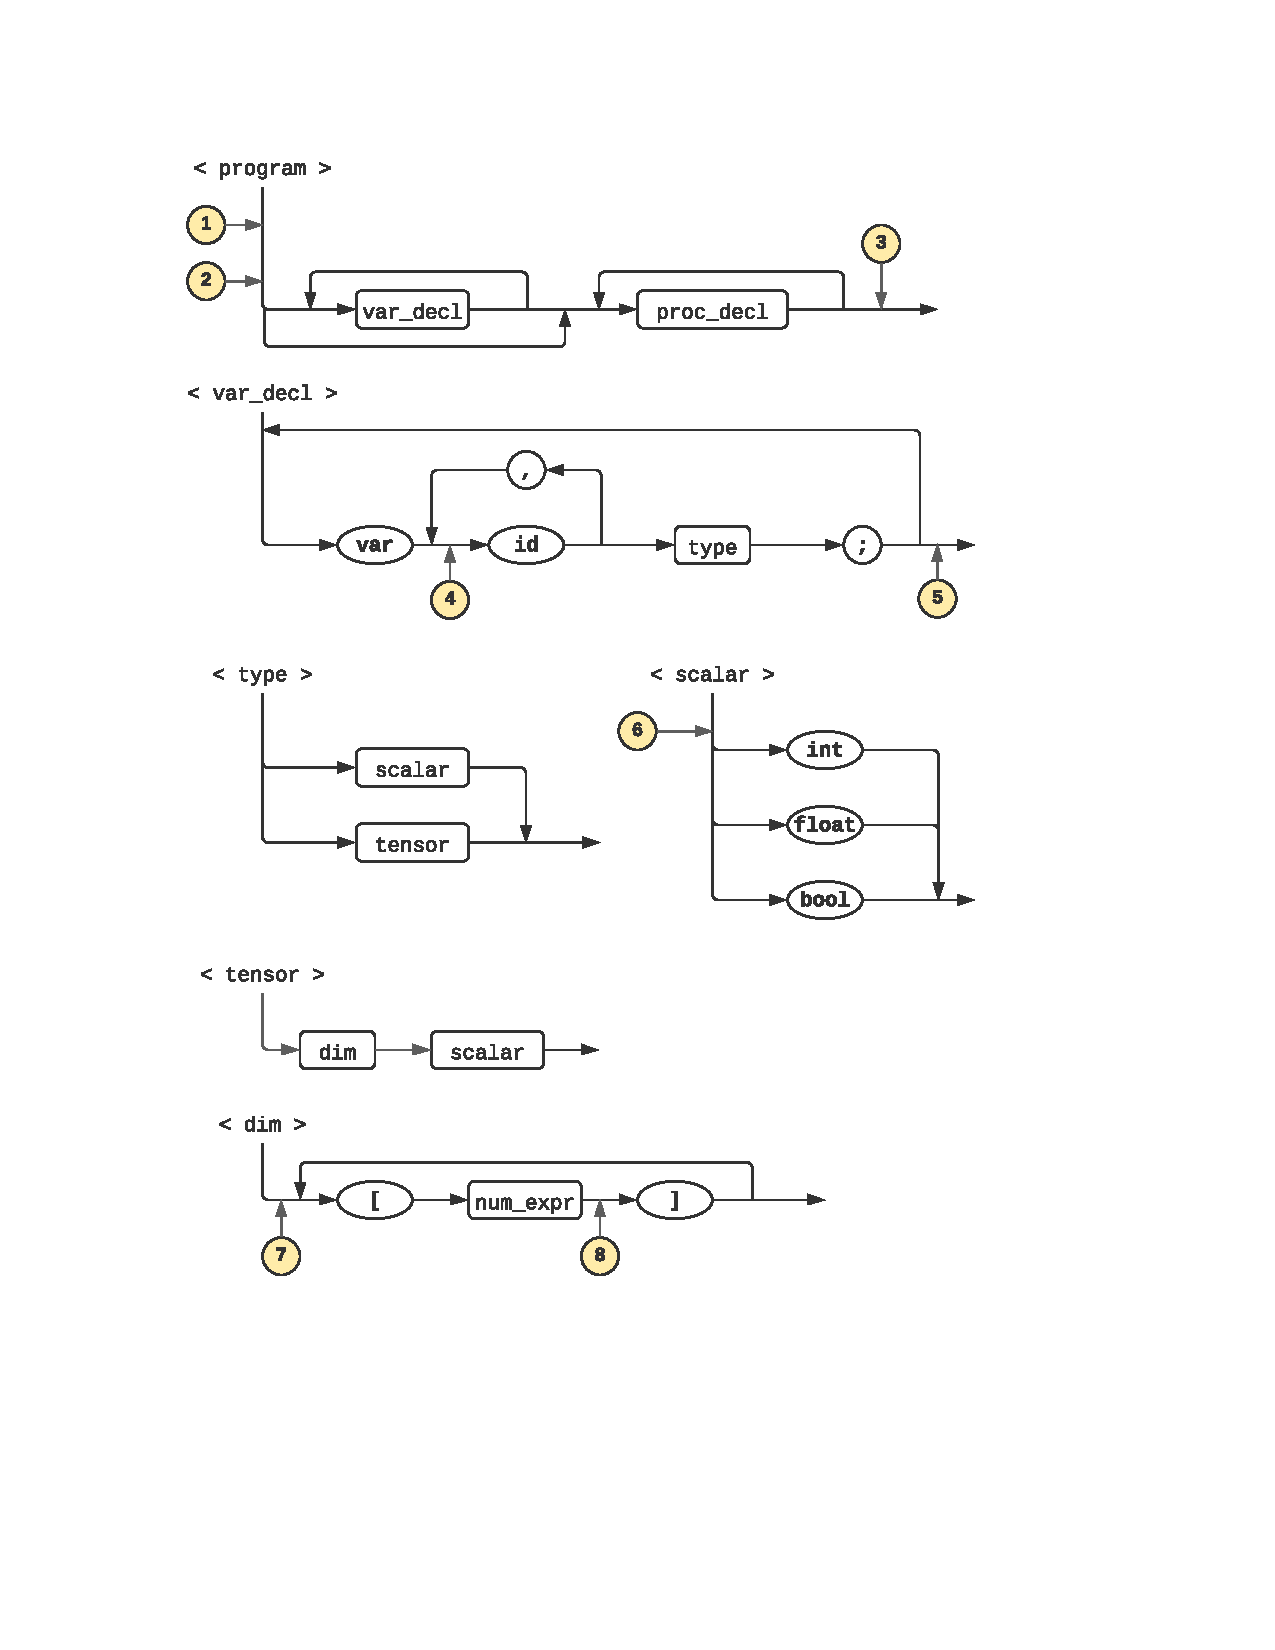
\includegraphics[
        trim={1in, 1in, 1in, 1in}, clip, page=1, scale=0.75]{diagrams/syntax}
\end{figure}
\newpage

\begin{figure}[H]
    \centering
    \begin{tabular}{cp{3in}}
        \toprule
        \textbf{No.} & \textbf{Description}\\
        \midrule 1 & Compiler initialization\\
        \midrule 2 & Generate era and goproc for starting procedure\\
        \midrule 3 & If valid program the create obj file\\
        \midrule 4 & If valid program the create obj file\\
        \midrule 5 & Turn on in\_decl flag\\
        \midrule 6 & Turn off in\_decl flag\\
        \midrule 7 & Turn off in\_decl flag\\
        \midrule 8 & Use dimqueue and symqueue to create symbols and add each
        to symbol table, if symbol has been read then raise error\\
        \bottomrule
    \end{tabular}
\end{figure}

\newpage

\begin{figure}[H]
    \centering
    \includegraphics[
        trim={1in, 1in, 1in, 1in}, clip, page=2, scale=0.75]{diagrams/syntax}
\end{figure}
\newpage

\begin{figure}[H]
    \centering
    \begin{tabular}{cp{3in}}
        \toprule
        \textbf{No.} & \textbf{Description}\\
        \midrule  9 & Add id to symbol table, if symbol has been read then
        raise error\\
        \midrule 10 & Update procedure's parameter information, argc and
        ret\_type\\
        \midrule 11 & Generate endproc, update procedure's type counters,
        resolve recursive calls, and clear scope\\
        \midrule 12 & Turn on in\_decl and in\_args flags\\
        \midrule 13 & Push id to symqueue\\
        \midrule 14 & Register return type\\
        \midrule 15 & Push or to opstack\\
        \midrule 16 & Push and to opstack\\
        \midrule 17 & If or at top of opstack then GenerateOpTac\\
        \bottomrule
    \end{tabular}
\end{figure}

\newpage

\begin{figure}[H]
    \centering
    \includegraphics[
        trim={1in, 1in, 1in, 1in}, clip, page=3, scale=0.75]{diagrams/syntax}
\end{figure}
\newpage

\begin{figure}[H]
    \centering
    \begin{tabular}{cp{3in}}
        \toprule
        \textbf{No.} & \textbf{Description}\\
        \midrule 18 & Push LPAREN to opstack\\
        \midrule 19 & Push RPAREN to opstack\\
        \midrule 20 & Push \#t to argstack and push bool\_t to typestack\\
        \midrule 21 & Push \#f to argstack and push bool\_t to typestack\\
        \midrule 22 & If and at top of opstack then GenerateOpTac\\
        \midrule 23 & If not at top of opstack then GenerateOpTac\\
        \midrule 24 & GenerateOpTac\\
        \bottomrule
    \end{tabular}
\end{figure}

\paragraph{Note} Keep in mind actions 18 and 19, since they are reused.

\newpage

\begin{figure}[H]
    \centering
    \includegraphics[
        trim={1in, 1in, 1in, 1in}, clip, page=4, scale=0.75]{diagrams/syntax}
\end{figure}
\newpage

\begin{figure}[H]
    \centering
    \begin{tabular}{cp{3in}}
        \toprule
        \textbf{No.} & \textbf{Description}\\
        \midrule 25 & Push + to opstack\\
        \midrule 26 & Push --- to opstack\\
        \midrule 27 & Push * to opstack\\
        \midrule 28 & Push / to opstack\\
        \midrule 29 & If + or --- at top of opstack then GenerateOpTac\\
        \midrule 30 & Push int literal to argstack push int\_t to typestack\\
        \midrule 31 & Push float literal to argstack push float\_t to typestack\\
        \midrule 32 & If * or / at top of opstack then GenerateOpTac\\
        \midrule 33 & Push id to argstack and its type to typestack\\
        \midrule 34 & If id dimension is 0 then raise error else push LPAREN\\
        \midrule 35 & Push RPAREN to opstack, if curr\_dim is different from
        expected dimension then raise error\\
        \bottomrule
    \end{tabular}
\end{figure}

\newpage

\begin{figure}[H]
    \centering
    \includegraphics[
        trim={1in, 1in, 1in, 1in}, clip, page=5, scale=0.75]{diagrams/syntax}
\end{figure}
\newpage

\begin{figure}[H]
    \centering
    \begin{tabular}{cp{3in}}
        \toprule
        \textbf{No.} & \textbf{Description}\\
        \midrule 36 & Init paramc,  if curr\_pcall is empty then assign 
        id to curr\_pcall else raise error, if exists in symtable the generate
        era else raise error\\
        \midrule 37 & Push RPAREN to opstack, GenerateParamTac\\
        \midrule 38 & if has return value then GenereteReturnTac else if
        in\_stmt Generate goproc, if paramc different from procedures argc
        then raise error\\
        \midrule 39 & Turn on in\_stmt flag\\
        \midrule 40 & Turn off in\_stmt flag\\
        \bottomrule
    \end{tabular}
\end{figure}

\newpage

\begin{figure}[H]
    \centering
    \includegraphics[
        trim={1in, 1in, 1in, 1in}, clip, page=6, scale=0.75]{diagrams/syntax}
\end{figure}
\newpage

\begin{figure}[H]
    \centering
    \begin{tabular}{cp{3in}}
        \toprule
        \textbf{No.} & \textbf{Description}\\
        \midrule 41 & Push $\leftarrow$ to opstack\\
        \midrule 42 & GenerateOpTac\\
        \midrule 43 & Push pc to jmpstack and GenerateJmpTac (JMF)\\
        \midrule 44 & Pop jmpstack and use value fo FillJmpTac\\
        \midrule 45 & Push pc to jmpstack and FillJmpTac\\
        \midrule 46 & Pop jmpstack and use value fo FillJmpTac\\
        \midrule 47 & Increment loop\_nest\\
        \midrule 48 & Fill unresolved jumps according loop style, fill skips and
        breaks, decrement loop\_nest\\
        \midrule 49 & Push pc to jmpstack and set loopstyle to ForStyle\\
        \midrule 50 & Push pc to jmpstack, GenerateJmpTac (JMT), push pc to 
        jmpstack and GenerateJmpTac (JMP)\\
        \midrule 51 & Push pc to jmpstack\\
        \midrule 52 & GenerateJmpTac (JMP), handle jumps for condition when
        true, false, and return from control variable assignment\\
        \midrule 53 & Push pc to jmpstack and set loopstyle to WhileStyle\\
        \midrule 54 & Push pc to jmpstack and GenerateJmpTac (JMF)\\
        \midrule 55 & Push pc to jmpstack and set loopstyle to InfLoop\\
        \bottomrule
    \end{tabular}
\end{figure}

\newpage

\begin{figure}[H]
    \centering
    \includegraphics[
        trim={1in, 1in, 1in, 1in}, clip, page=7, scale=0.75]{diagrams/syntax}
\end{figure}
\newpage

\begin{figure}[H]
    \centering
    \begin{tabular}{cp{3in}}
        \toprule
        \textbf{No.} & \textbf{Description}\\
        \midrule 56 & Push break or skip to its appropiate queue, GenerateJmpTac
        (JMP)\\
        \midrule 57 & GenerateRetTac\\
        \midrule 58 & Change last PRINT to PRINTLN\\
        \midrule 59 & GeneratePrintTac\\
        \midrule 60 & Pop argstack and typestack and use values to generate
        read TAC\\
        \bottomrule
    \end{tabular}
\end{figure}

\newpage

\begin{figure}[H]
    \centering
    \includegraphics[
        trim={1in, 1in, 1in, 1in}, clip, page=8, scale=0.75]{diagrams/syntax}
\end{figure}
\newpage

\begin{figure}[H]
    \centering
    \begin{tabular}{cp{3in}}
        \toprule
        \textbf{No.} & \textbf{Description}\\
        \midrule 61 & Push unary function to opstack, GenerateOpTac and push
        RPAREN to opstack\\
        \bottomrule
    \end{tabular}
\end{figure}

\newpage

\begin{figure}[H]
    \centering
    \includegraphics[
        trim={1in, 1in, 1in, 1in}, clip, page=9, scale=0.75]{diagrams/syntax}
\end{figure}
\newpage

\begin{figure}[H]
    \centering
    \begin{tabular}{cp{3in}}
        \toprule
        \textbf{No.} & \textbf{Description}\\
        \midrule 62 & Push binary function to opstack, GenerateOpTac and push
        RPAREN to opstack\\
        \midrule 63 & If variable exists and has appropiate dimensions then
        push vec function to opstack, GenerateOpStack\\
        \bottomrule
    \end{tabular}
\end{figure}

\newpage
\subsection{Semantic Consideration Table}
\newpage

\section{Memory Management}
\subsubsection{Tree listener}
\begin{figure}[h]
    \centering
    \begin{tabular}{p{1in}p{3in}}
        \toprule
        \textbf{Element} & \textbf{Description}\\
        \midrule filename &
        Keeps the name of the source code to produce the executable.\\

        \midrule valid &
        Flag to indicate whether an error has been found or not.\\

        \midrule debug &
        Flag to indicate whether debug mode is toggled.\\

        \midrule symtable &
        Table to keep track of the variable symbols and procedures used in
        source code.\\

        \midrule symqueue &
        Queue to keep track of which symbols are under the same declaration list.\\

        \midrule typequeue &
        Queue to keep track of which symbols are under the same declaration line.\\

        \midrule paramqueue &
        Queue to keep track of which symbols are on the procedures parameters.\\

        \midrule dimmqueue &
        Queue to keep track of which the dimensions used by a tensor.\\

        \midrule in\_decl &
        Flag to know if it is reading a variable declaration.\\

        \midrule in\_args &
        Flag to know if it is reading the arguments of a procedure.\\

        \midrule in\_stmt &
        Flag to know if it is reading a statement.\\

        \midrule scope &
        Flag to know the current scope.\\

        \midrule argc &
        Counter for arguments used in a procedure call.\\

        \midrule loop\_nest &
        Counter to keep track of loop nesting.\\

        \midrule ret\_type &
        Variable to keep track of current procedure's \newline return type.\\

        \midrule curr\_proc &
        Variable to keep track of the name of current \newline procedure.\\

        \bottomrule
    \end{tabular}\\
\end{figure}

\begin{figure}[H]
    \centering
    \begin{tabular}{p{1in}p{3in}}
        \toprule
        \textbf{Element} & \textbf{Description}\\
        \midrule ir\_code &
        Array of TACs (three-address code) generated by the compiler.\\

        \midrule data\_seg &
        Array of TACs used for data segment generated by the compiler.\\

        \midrule op\_stack &
        Stack of operators for expression compilation.\\

        \midrule arg\_stack &
        Stack of arguments for operators for expression compilation.\\

        \midrule type\_stack &
        Stack of type variables for expression compilation.\\

        \midrule pc &
        Program counter to keep track of generated TACs.\\

        \midrule tmpc &
        Temporal counter to keep track of generated \newline temporal variables.\\

        \midrule tmpc &
        Temporal counter to keep track of generated \newline temporal variables.\\

        \midrule paramc &
        Parameter counter to keep track of number of \newline parameters given
        to a procedure.\\

        \midrule loopstyle &
        Variable to keep track of which kind of loop syntax is used.\\

        \midrule startpoint &
        Variable to keep track of where to start the \newline program.\\

        \midrule startproc &
        Variable to keep track of the name of initial \newline procedure.\\

        \midrule curr\_line &
        Variable to keep track of current line.\\

        \midrule curr\_column &
        Variable to keep track of current column.\\

        \midrule curr\_pcall &
        Variable to keep track of the name of current \newline procedure call.\\

        \midrule curr\_tensor &
        Variable to keep track of the name of current \newline tensor in use.\\

        \midrule curr\_dim &
        Variable to keep track of the name of current \newline dimension 
        index used in tensor indexing.\\

        \midrule memmap &
        Memory mapper, to assign a memory address to a used variable.\\

        \bottomrule
    \end{tabular}\\
\end{figure}

\newpage

\subsubsection{Symbol}

\begin{figure}[H]
    \centering
    \begin{tabular}{p{1in}p{3in}}
        \toprule
        \textbf{Element} & \textbf{Description}\\
        \midrule Stype &
        Enumeration to indicate the type of a variable.\\

        \midrule Dim &
        Array to keep track of the dimensions of a variable.\\

        \midrule Baddress &
        Base address, to keep track of base address for tensiorial types.\\

        \midrule Argc &
        Argument count, to keep track of the arguments required for procedure.\\

        \midrule TypeArgs &
        Array to keep track of the number of arguments of a procedure.\\

        \midrule RetType &
        Variable to keep track of the return type of an argument.\\

        \midrule Startpoint &
        Variable to keep track of the starting point of a procedure.\\

        \midrule Paddress &
        Parameter address, array to keep track of the reserved addresses for
        the parameter.\\

        \midrule Type count &
        Counters for the amount of variables of each type required.\\

        \bottomrule
    \end{tabular}\\
\end{figure}

\subsubsection{Symbol Table}

\begin{figure}[H]
    \centering
    \begin{tabular}{p{1in}p{3in}}
        \toprule
        \textbf{Element} & \textbf{Description}\\
        \midrule table &
        An array of size 2 of hash tables that take strings as keys and Symbols
        as values.\\

        \bottomrule
    \end{tabular}\\
\end{figure}

\subsubsection{Memory mapper}

\begin{figure}[H]
    \centering
    \begin{tabular}{p{1in}p{3in}}
        \toprule
        \textbf{Element} & \textbf{Description}\\
        \midrule memcache &
        Hash table of strings as keys and int as value, to store every symbol
        with a memory address.\\

        \midrule Typecount &
        An array of size 2 of hash table that takes strings as keys and ints as
        values, to store a counter of used memory per scope and type.\\

        \bottomrule
    \end{tabular}\\
\end{figure}
